\subsection{Workflow}
\label{s:ProblemDomain:Workflow}

Workflow is an application comprising of a set of tasks, where some of them are dependent one on another and all need to be processed in order to complete workflow's objective and yield the final results.
Each job in such pipeline may require its own input data to begin execution and returns an output, when it ends successfully.
As tasks cannot start without their input, they need to wait for results from other tasks, which creates a dependency relationship.
This allows such applications to be represented in a form of a \emph{Directed Acyclic Graph (DAG)} as shown in \cref{fig:workflow:dag-example}.

Furthermore, not all the jobs in a workflow must perform the same set of operations at runtime.
The pipeline has the layered structure where each layer represents the groups of tasks independent of each other.
This allows for a straightforward data-parallel task execution within a single layer. 


%%%%
\begin{figure}[H]
\centering
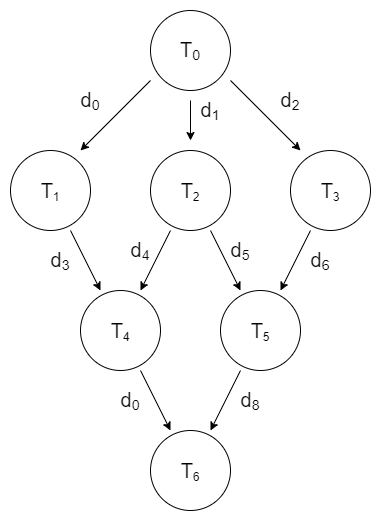
\includegraphics[width=0.3\linewidth]{figures/2-3-dag-example-with-d.png}
\caption{Exemplary workflow application structure}
\label{fig:workflow:dag-example}

\smallskip
\begin{minipage}{0.6\textwidth}
{\footnotesize
Tasks are presented as a \emph{T\textsubscript{i}} nodes and dependencies as a \emph{d\textsubscript{j}} edges. 
\par}
\end{minipage}

\end{figure}
%%%%


There are applications with more than one starting or finishing jobs, however their representations can have a single abstract nodes prepended or appended, in order to match the input for scheduling algorithms.



\subsubsection{Montage}

One of the scientific workflows integrated with Hyperflow system is \emph{Montage}.
It is a toolkit that provides transformations for the astronomical images to turn them into the custom, science-grade mosaics \cite{b:Montage-url}.
Each transformation is provided as a separate software module \cite{b:Montage} so together they can be piped into a single workflow.



\subsubsection{SoyKB}

The \emph{Soybean Konwledge Base (SoyKB)} is a platform for storing soybean genomics datasets and providing them via an interface for the research.
To analyze this data the \emph{PGen workflow} was created allowing analysis on both Linux environment and through SoyKB online submissions \cite{b:SoyKB-workflow-url, b:SoyKB-PGen}.
% The latter environment integration allows execution of the workflow with task containerization.
Being consistent with Hyperflow naming, in this work all mentions of \emph{SoyKB workflow} are in fact referring to the PGen application.


